% Created 2020-11-02 seg 11:24
% Intended LaTeX compiler: pdflatex
\documentclass[11pt]{article}
\usepackage[utf8]{inputenc}
\usepackage{lmodern}
\usepackage[T1]{fontenc}
\usepackage[top=3cm, bottom=2cm, left=3cm, right=2cm]{geometry}
\usepackage{graphicx}
\usepackage{longtable}
\usepackage{float}
\usepackage{wrapfig}
\usepackage{rotating}
\usepackage[normalem]{ulem}
\usepackage{amsmath}
\usepackage{textcomp}
\usepackage{marvosym}
\usepackage{wasysym}
\usepackage{amssymb}
\usepackage{amsmath}
\usepackage[theorems, skins]{tcolorbox}
\usepackage[style=abnt,noslsn,extrayear,uniquename=init,giveninits,justify,sccite,
scbib,repeattitles,doi=false,isbn=false,url=false,maxcitenames=2,
natbib=true,backend=biber]{biblatex}
\usepackage{url}
\usepackage[cache=false]{minted}
\usepackage[linktocpage,pdfstartview=FitH,colorlinks,
linkcolor=blue,anchorcolor=blue,
citecolor=blue,filecolor=blue,menucolor=blue,urlcolor=blue]{hyperref}
\usepackage{attachfile}
\usepackage{setspace}
\usepackage{tikz}
\author{Gabriel Petrini da Silveira}
\date{\today}
\title{}
\begin{document}

\tableofcontents


A growing body of empirical demand-led literature has evaluated the role of NCC autonomous expenditures.
\textcite{freitas_pattern_2013} present a growth accounting decomposition fro Brazil from 1970 to 2005 and report the relevance of those expenditures in describing Brazilian GDP growth. \textcite{braga_investment_2018} shows evidence that economic growth and non-residential investment are explained by NCC autonomous expenditures in Brazilian economy from 1962 to 2015. For the U.S., \textcite{girardi_long-run_2016} show that NCC autonomous expenditures have permanent effects on growth rate. 
\textcite{haluska_growth_2019} employ Granger-causality tests to assess the stability of the SSM for the US (1987-2017) and report a causality from NCC autonomous expenditures to the marginal propensity to invest, as expected.
Finally, \textcite{girardi_autonomous_2018} bring evidence that those expenditures determine investment share on GDP for twenty OECD countries.

However, there still is a lack of studies on the role of residential investment specifically.
What is commonly  discussed about this NCC autonomous expenditure is largely based on \textcite{green_follow_1997} pioneer work.
Based on Granger Causality and cointegration tests for the US from 1959-1992, this is one of the first papers to indicates that residential investment leads the business cycle.
Subsequently, \textcite{leamer_housing_2007} concludes that this pattern occurs at least since the post-war period.
More precisely,  \textcite[p.~8]{leamer_housing_2007} describes US business cycles as follows: ''[f]irst homes, then cars,
and last business equipment''.
Recently, \textcites{fiebiger_semi-autonomous_2018}{fiebiger_trend_2017} also report residential investment as an important determinant of business cycles for the US based on causal narratives.

After the Great Recession (2008-2009), there has been growing macroeconometric studies on housing.
However, most of them have emphasized house prices and not its volume (residential investment).
\textcite{goodhart_house_2008} for instance, estimate a time-series fixed effects panel data for 17 industrialized countries from 1970 to 2006. They report a multidirectional relation between money, credit, house prices and GDP growth and have found stronger effects during housing booms\footnote{\textcite{Arestis_Bank_2014} also found a  direct relationship between house prices and credit volume based on cointegration and error correction techniques for 9 OECD countries from 1970 to 2011.}. 
\textcite{wood_house_2020} report that house prices are relevant for describing household indebtedness from 1980 to 2017 in 18 advance economies.
However, both studies do not include residential investment.
\textcite{arestis_residential_2015}, on the other side, include residential investment. Using a ARDL model for 17 OECD countries from 1970 to 2013, the authors report that banking credit and real house prices are the most statistically significant variables for real residential investment in the US.
Although those approaches are interesting, it fails to take into account the connection between asset bubbles and aggregate demand which is relevant for describe the recent housing burst event.

From this review of recent empirical literature, it is noticeable that few macroeconometric studies have investigated residential investment in any systematic way.
In this paper, we argue that besides this growing body of literature that recognizes the macroeconomic importance of residential investment, little progress has been made in understanding its theoretical determinants.
On the following subsection, we present some residential investment-related stylized facts in order to highlight its relevance for the US business cycle which will be compared to the theoretical model in Section \ref{real_sim}.
Next, we analyze the connection between residential investment, real estate inflation and mortgage interest rate during the U.S. housing bubble episode.



\section{Residential investment stylized facts}
\label{sec:orge149a9d}

As discussed before, both \textcites{green_follow_1997}{leamer_housing_2007} made it clear how important this particular expenditure is to USA business cycle. In this subsection, we show some residential investment stylized facts for the US in more detail.

\begin{itemize}
\item[{$\square$}] Introdução mais alongada
\end{itemize}

Figure \ref{Investo_Resid_GDP} shows how residential investment movements help to predict recessions. Recessions are anticipated by a reduction of residential investment share on GDP, while the expansion of those expenditures precedes economic recovery. The fall of dwellings expenditures in 1966-67 are an exception because the increase of military expenditures because of Vietnam War offset an eventual economic downturn \cite[p.~20]{leamer_housing_2007}. Another exception is the dot-com bubble 2000 crisis that was not caused by residential investment. The Great Recession 2008-2009 is the one in which this pattern is the most evident. 



\begin{figure}[htb]
    \centering
        \caption{Residential Investment as share of GDP}
        \label{Investo_Resid_GDP}
    \includegraphics[width = 0.7\textwidth]{./figs/res_share.png}
    \caption*{\textbf{Source:} Federal Reserve Bank of St. Louis, authors’ elaboration}
\end{figure}

In order to depict the relation between housing and business cycle, we present Figure \ref{fig:cycles} in which each cycle is represented in a different panel\footnote{Similar reasoning can be found in \textcite{fiebiger_trend_2017}. Unlike them, we plot only residential investment without including other households expenses financed by credit.}.
Residential investment-GDP ratio and capacity utilization --- as a proxy for business cycle --- are presented on vertical and horizontal axis respectively.
Economic recovery is generally characterized by residential investment growing faster than GDP\footnote{It worth noting that 1991-2000 period is a particular case.}. Both residential investment share on GDP and capacity utilization increase as a consequence of higher growth rate.
Following the Sraffian supermultiplier growth model, we conclude that increase of non-residential investment is the result of capital stock adjustment principle. This increase implies GDP to grow faster than residential investment, therefore reducing both its share on GDP and capacity utilization ratio. Finally, as a result of economic burst, capacity utilization ratio falls and the cycle ends.



\begin{figure}[htb]
    \centering
        \caption{Share of residential investment and capacity utilization during business cycles\\\centering (Dots size grow in  time)} 
    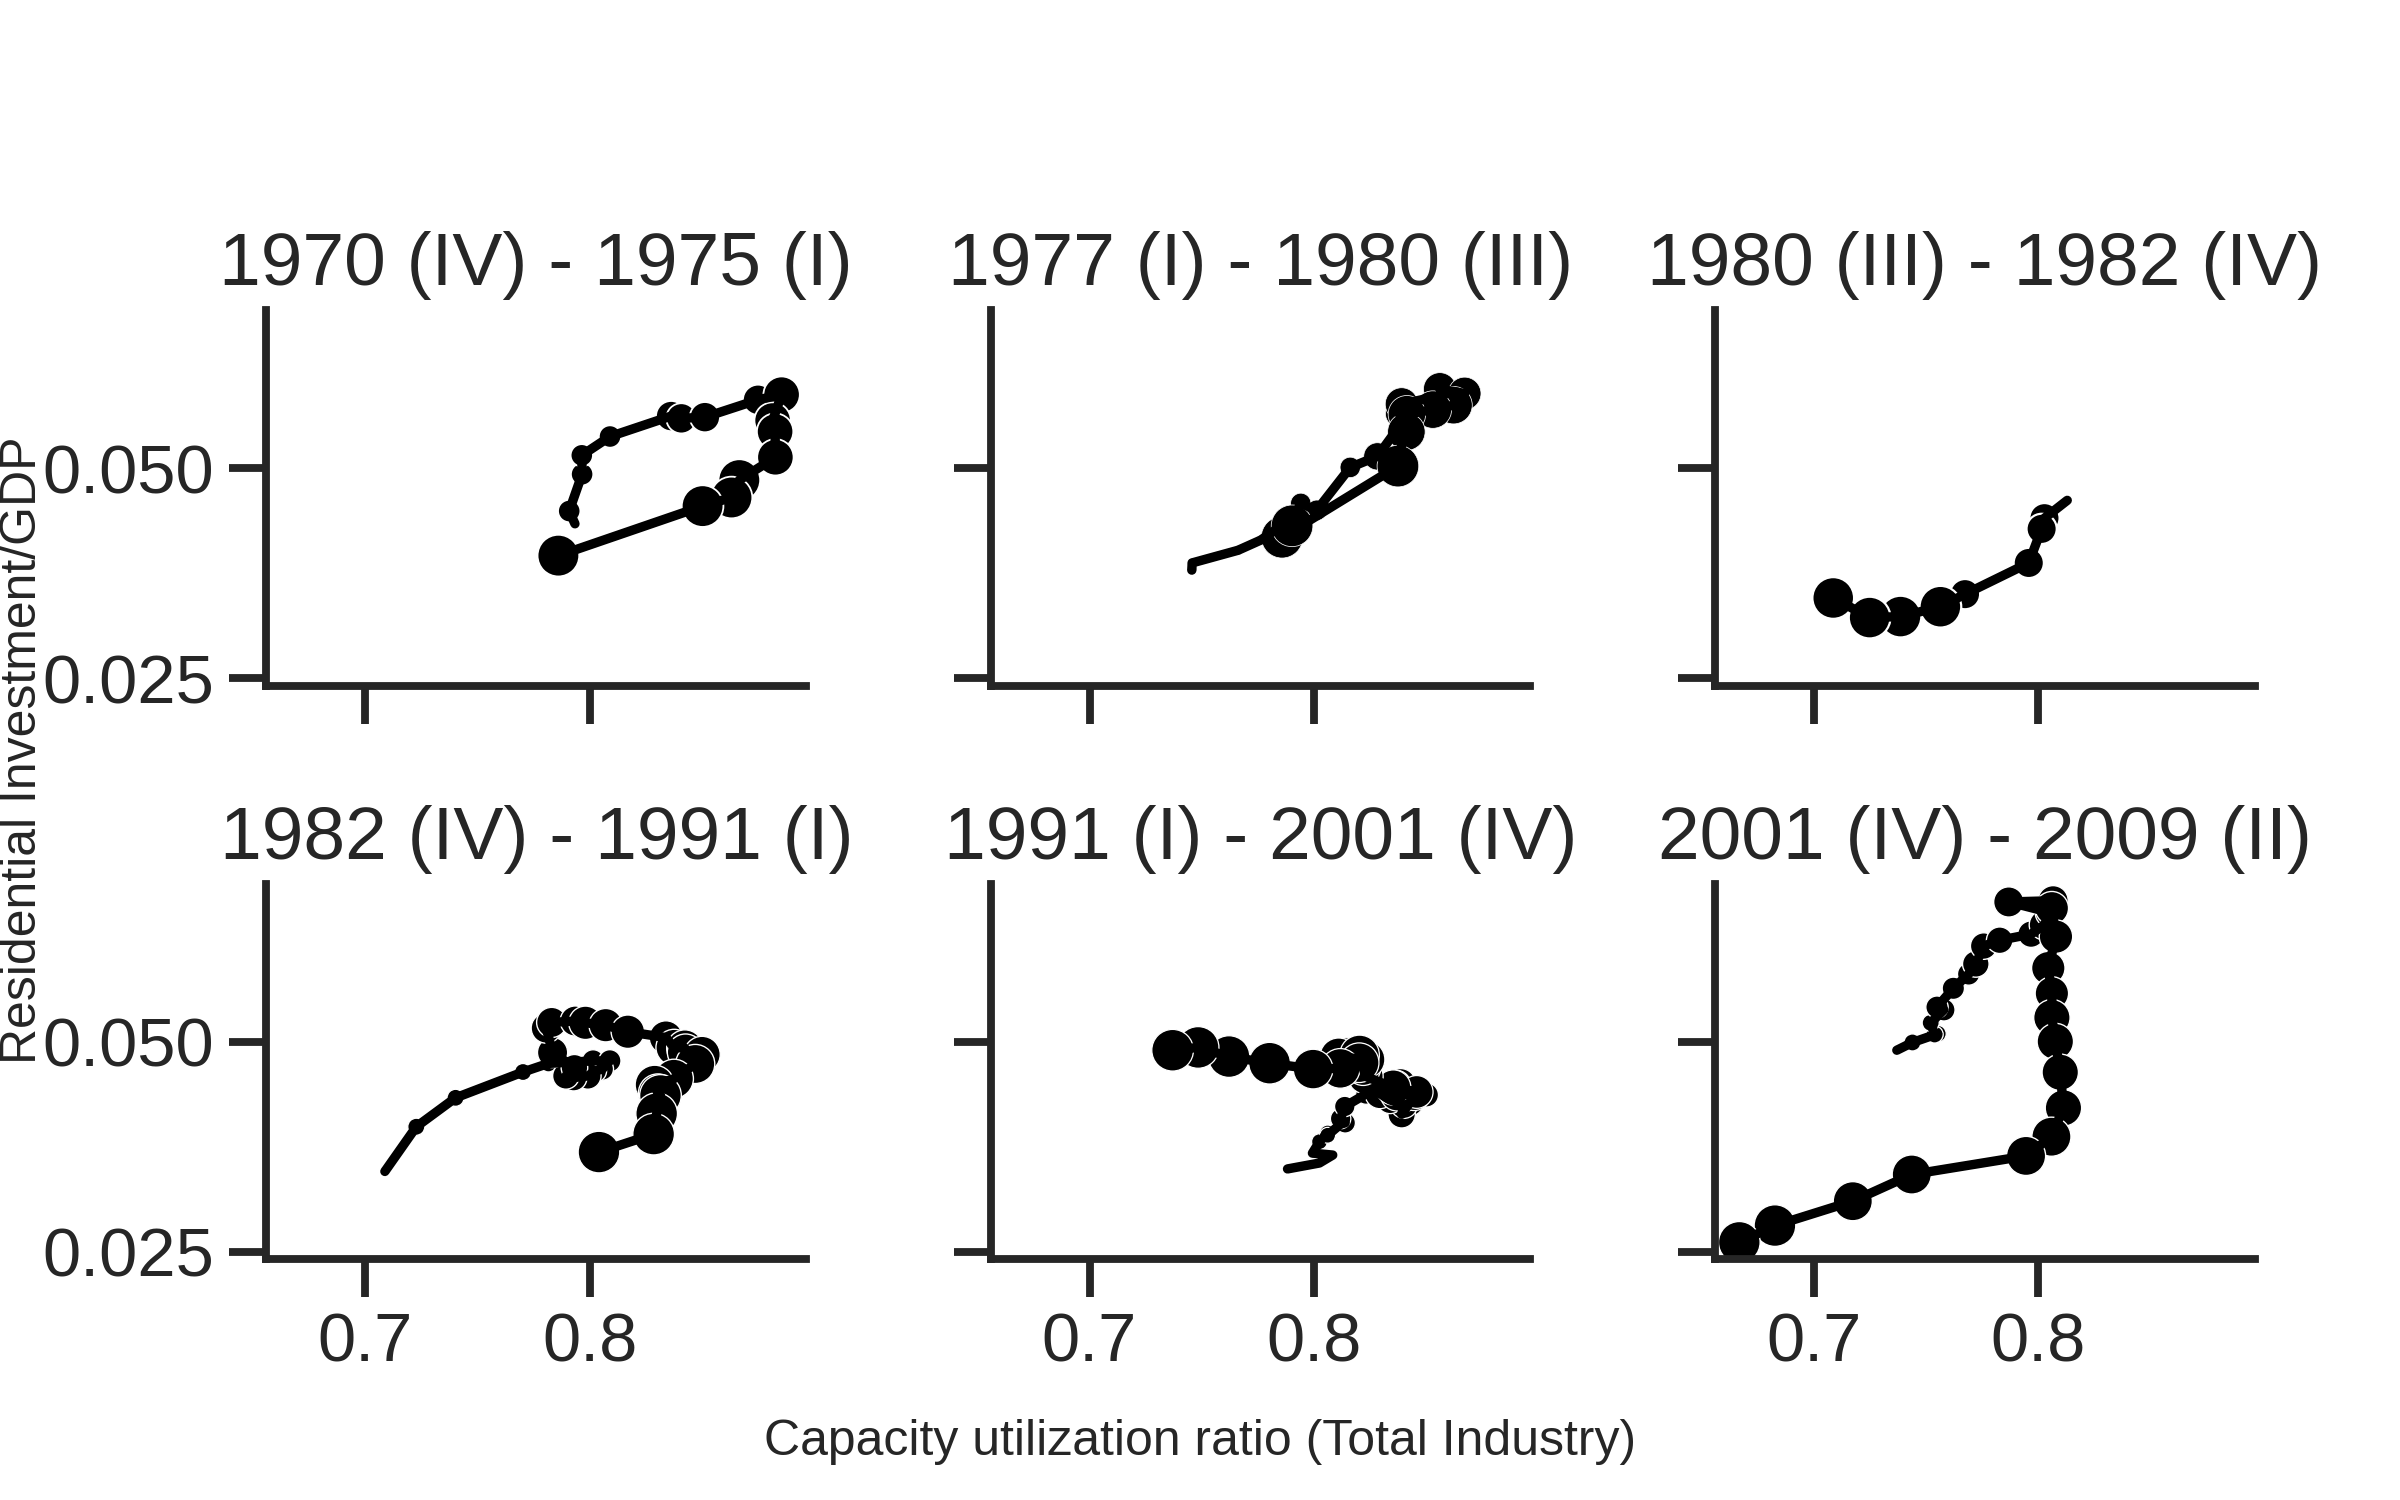
\includegraphics[width = 0.9\textwidth]{./figs/cycles.png}
    \label{fig:cycles}
    \caption*{\textbf{Source:} Federal Reserve Bank of St. Louis, authors’ elaboration.}
\end{figure}
Additionally, some key aspects of recent housing developments have not been dealt with in depth.
More specifically, there has been little discussion on popularization of primary houses and concentration of secondary ones\footnote{According to \textcite{us_census_bureau_characteristics_2017}, a primary property is one that the owner has regular access to and, in the case of having more than one (secondary) property, it is the one that enjoys most of the time throughout the year. Secondary properties are those where:
(i) the owners reside part of the year only; (ii) it is at least 50 miles from the primary property and; (iii) cannot be subject to a rental agreement.}. The expansion of primary houses can be seen in Figure \ref{fig:concentration}, which shows concentration curves from 1989 to 2010 by different types of properties (primary and secondary)\footnote{Concentration curves are drawn from the cumulative ordering of two distinct variables. The horizontal axis of Figure \ref{fig:concentration} contains the cumulative proportion of wealthy households while the vertical axis shows the accumulated proportion of a portion of this wealth (in this case, primary and secondary houses). Finally, to build the concentration curves, both axes are ordered by total wealth. Thus, unlikely the Lorenz curve, concentration curves are non-decreasing. As a consequence, it can cross the perfect equality line. For more details, see \textcite{Jann_Concentration_2016}.}. Based on these curves, it is possible to assess how concentrated a certain asset is by comparing it with perfect equality line\footnote{In 2010, for example,  up to 25\% of wealthy households owned 21.80\% of all primary houses. Moving on, households up to 50\%, 75\% and 90\% owned 61.30\%, 90.10\% and  95.30\% respectively while 2.9\% was not in the possession of any households.}\textsuperscript{,}\,\footnote{The higher and to the left a concentration curve is compared to the Lorenz curve, the less concentrated the asset is. In this case, the asset  is distributed in favor of the poorest strata of wealth. A concentration curve more to the right and below compared to the Lorenz curve indicates the opposite.}.

\begin{figure}[htb]
    \centering
        \caption{Concentration curves for primary and secoundary houses} 
    \includegraphics[width = 0.95\textwidth]{./figs/Concentration_Curve.png}
    \label{fig:concentration}
    \caption*{\textbf{Source:} Survey of Consumer Finance, authors’ elaboration.}
\end{figure}


A brief inspection of Figure \ref{fig:concentration} reveals that the years leading up to the Great Recession were characterized by the deconcentration of primary houses. In other words, poorer strata of the population now have a larger accumulated share of primary houses. 
Since this asset is mainly acquired for non-speculative reasons, there is a general increase in the demand for properties as final good. The same cannot be said about secondary houses whose concentration/distribution movement is not as marked as in the previous case. Since this type of property is not intended for regular use by its owner, deconcentration of this asset suggests an increase in the demand for properties in the expectation of capital gains\footnote{This increase in demand for secondary houses may indicate --- but is not limited to --- an increase for speculative reasons. A vacation or rental home, for example, are non-speculative uses of a secondary house. Nevertheless, it is argued that there is a connection between secondary houses and speculation with real estate. It worth noting that the wealthiest households are not the main holders of this secoundary houses. According to Figure \ref{fig:concentration}, they accumulate less than 50\% of these properties over the analyzed period (see vertical axis).}.

\subsection{Conexão com a subseção seguinte}
\label{sec:org873e117}


\begin{itemize}
\item[{$\square$}] Explicitar que os fatos estilizados apresentados até então serão comparados com o modelo teórico
\end{itemize}

\section{Housing bubble and residential investment}
\label{sec:orgfe7bcac}


After the Great Recession, the literature have analyzed the macroeconomic relevance of residential investment \cites{leamer_housing_2015}{fiebiger_semi-autonomous_2018}.
However, little progress has been made in understanding its theoretical determinants.
\textcite{teixeira_crescimento_2015} proposes the so-called houses own interest rate (\(own\)) in order to analyze the relation between residential investment, real estate inflation and interest rates during the U.S. housing bubble episode.
Estimated by deflating mortgages interest rate real estate inflation, this particular real interest rate is the most relevant for households since it is the real cost in real estate from buying real estate  \cite[p.~53]{teixeira_crescimento_2015}.
In short, this is the real interest rate that is relevant for house investors.
Figure \ref{propria_investo} shows how this  procedure is more adequate than a general price index deflation --- as \textcite[p.~143--6]{fair_macroeconometric_2013} does --- to describe residential investment growth rate\footnote{It is worth noting that during a housing bubble period, it is real estate inflation that governs own's interest rate dynamics. Therefore, the lower this rate is, the greater the capital gains (in real estate) for speculating with real estate will be. This negative relation between houses own interest rate and residential investment is shown in Figure \ref{propria_investo} in which this particular real interest rate has been gradually decreased over the real estate boom (2002-5).}.
Based on this concept, \textcite{petrini_demanda_2019} estimated an econometric model for the U.S. (1992 to 2019) and presents empirical evidence that the residential investment growth rate and houses own interest rate share a common negative long-run trend.
Furthermore, \textcite{petrini_demanda_2019} also reports a unidirectional long-run causality from houses own interest rate to residential investment growth rate.

EXPLICAR TAXA PRÓPRIA


\begin{figure}[htb]
	\centering
	\caption{Residential investment growth rate vs. Houses Own interest rate}
	\label{propria_investo}
	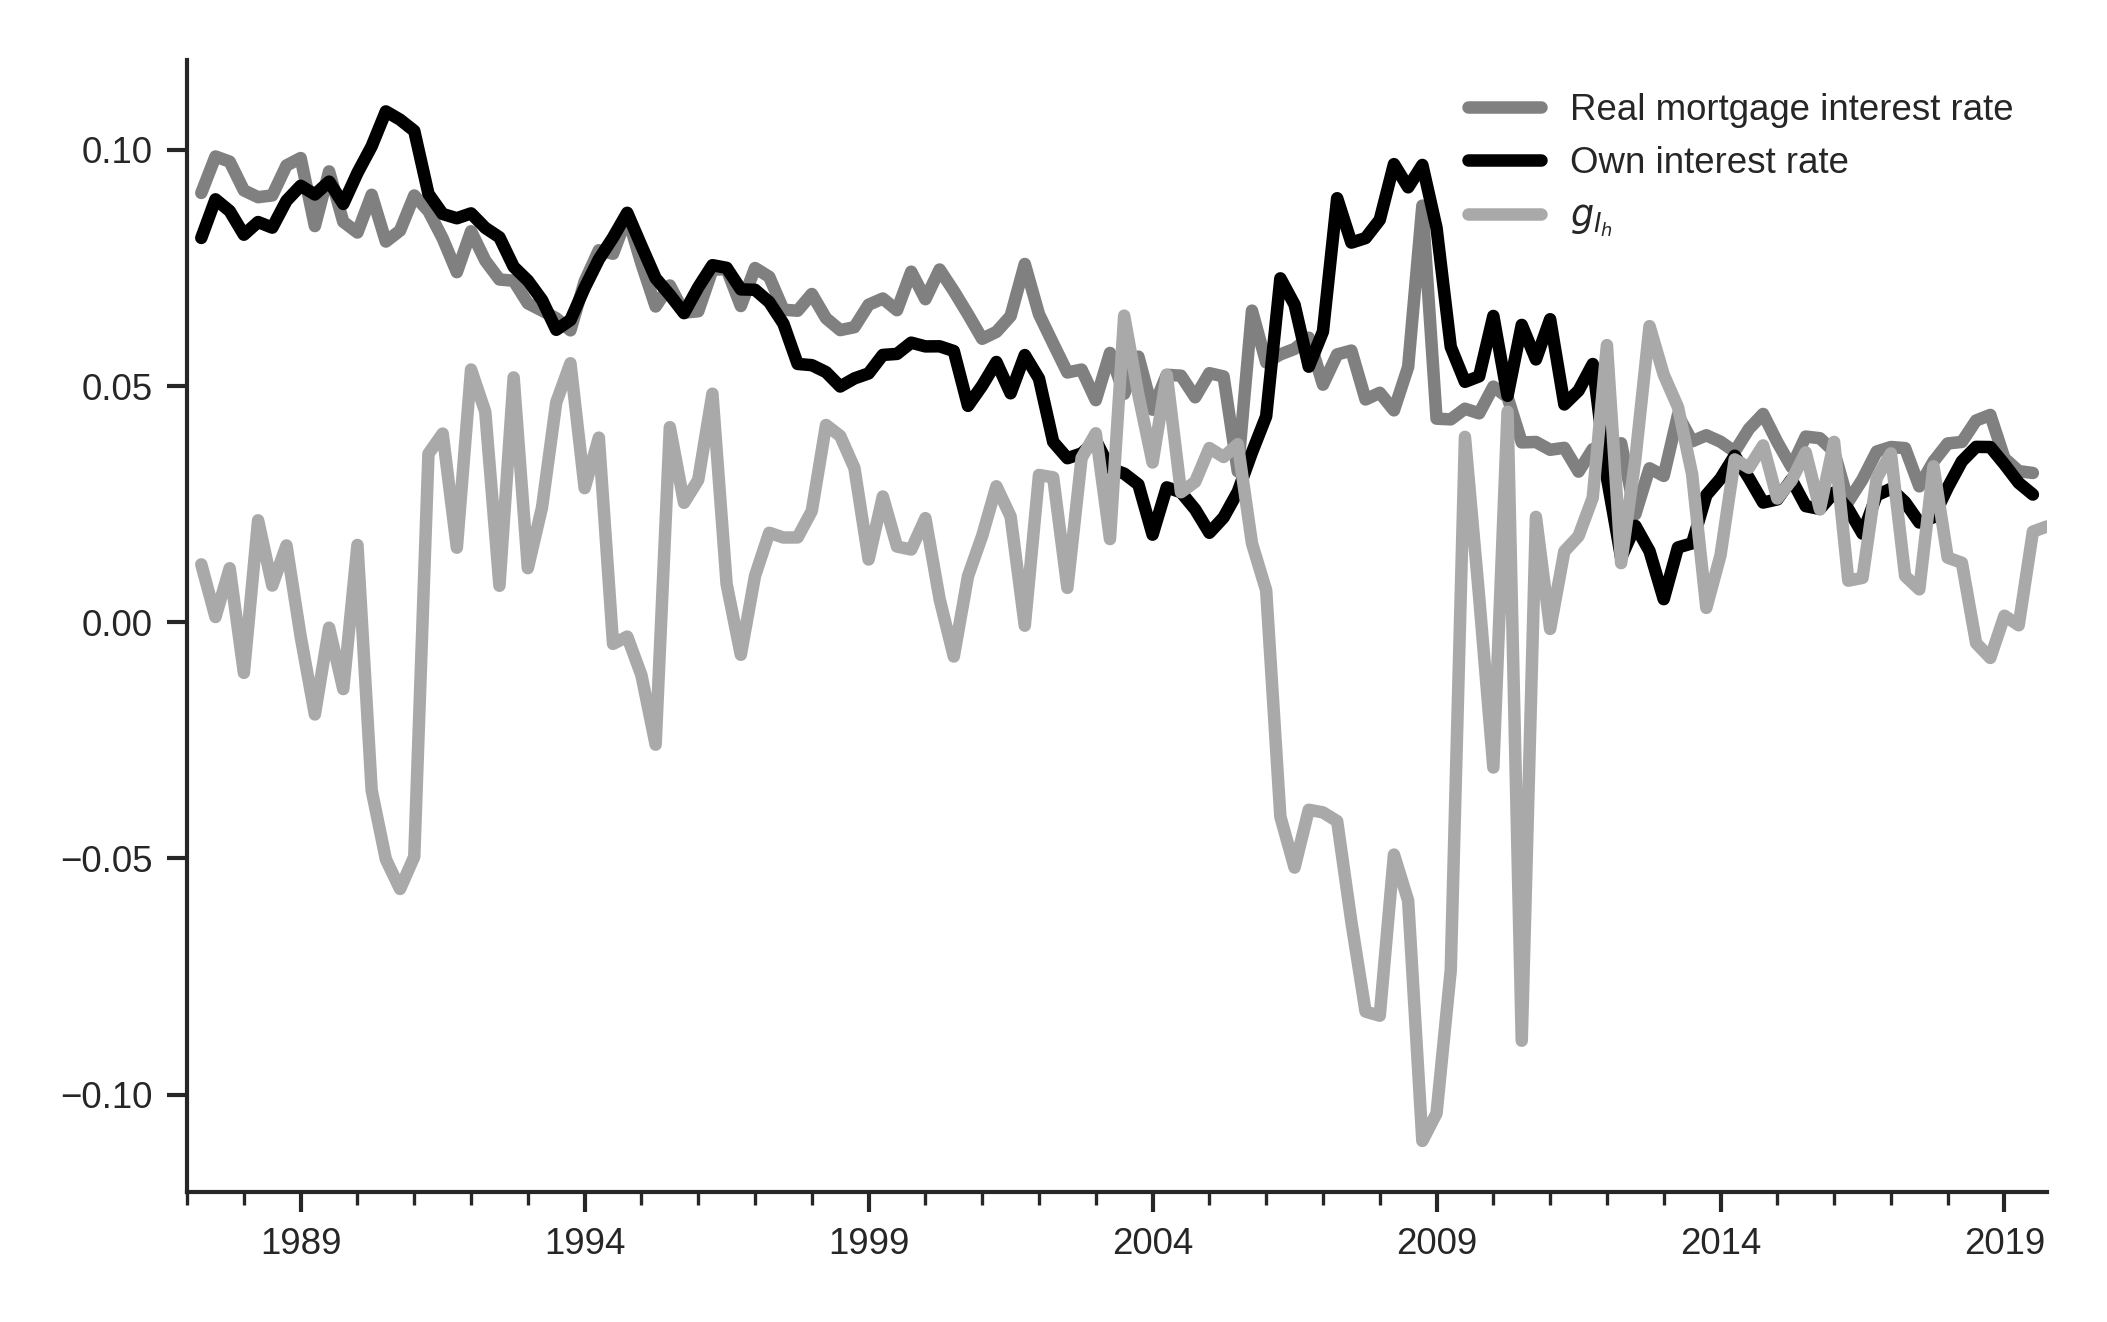
\includegraphics[width=.8\textwidth]{./figs/Own_gI}
	\caption*{\textbf{Source:} U.S. Bureau of Economic Analysis, Authors' elaboration}
\end{figure}





In summary, what we intended to show is that one cannot analyze the U.S. business cycle properly without considering residential investment and asset bubbles together.
\end{document}